% !TeX program = xelatex
% Journal-style author manuscript, not an official publisher class.
% Compile main.tex from this directory with XeLaTeX (twice) or Tectonic.
\documentclass[UTF8,a4paper,twocolumn,fontset=none,zihao=5]{ctexart}
\usepackage[top=20mm,bottom=20mm,left=18mm,right=18mm,columnsep=7mm]{geometry}
\usepackage{amsmath,amssymb,booktabs,graphicx,tabularx,array}
\usepackage{caption,enumitem,needspace,balance}
\usepackage{cite}
\newcommand{\upcite}[1]{\textsuperscript{\cite{#1}}}
\usepackage{xurl}
\usepackage[hidelinks,bookmarksnumbered]{hyperref}
\IfFontExistsTF{SimSun}{\setCJKmainfont{SimSun}[AutoFakeBold=2]}{\setCJKmainfont{FandolSong-Regular}[BoldFont=FandolSong-Bold]}
\IfFontExistsTF{SimHei}{\setCJKsansfont{SimHei}[AutoFakeBold=2]}{\setCJKsansfont{FandolHei-Regular}[BoldFont=FandolHei-Bold]}
\IfFontExistsTF{SimSun}{\setCJKmonofont{SimSun}}{\setCJKmonofont{FandolSong-Regular}}
\setmainfont{texgyretermes-regular.otf}[BoldFont=texgyretermes-bold.otf,ItalicFont=texgyretermes-italic.otf,BoldItalicFont=texgyretermes-bolditalic.otf]
\setsansfont{texgyreheros-regular.otf}[BoldFont=texgyreheros-bold.otf]
\ctexset{section={format=\large\sffamily\bfseries,beforeskip=9pt,afterskip=5pt},
 subsection={format=\normalsize\sffamily\bfseries,beforeskip=7pt,afterskip=3pt}}
\setlength{\parindent}{2em}
\setlength{\parskip}{0pt}
\linespread{1.04}
\setlength{\abovedisplayskip}{5pt plus 1pt minus 1pt}
\setlength{\belowdisplayskip}{5pt plus 1pt minus 1pt}
\setlength{\textfloatsep}{10pt plus 2pt minus 2pt}
\setlength{\dbltextfloatsep}{10pt plus 2pt minus 2pt}
\setlength{\floatsep}{8pt plus 2pt minus 2pt}
\renewcommand{\topfraction}{0.93}
\renewcommand{\dbltopfraction}{0.93}
\renewcommand{\textfraction}{0.06}
\renewcommand{\floatpagefraction}{0.80}
\renewcommand{\dblfloatpagefraction}{0.80}
\setcounter{topnumber}{3}
\setcounter{dbltopnumber}{3}
\makeatletter
\setlength{\@fptop}{0pt}
\setlength{\@fpsep}{10pt}
\setlength{\@fpbot}{0pt plus 1fil}
\makeatother
\captionsetup{font=small,labelsep=quad,skip=4pt}
\setlist[enumerate]{leftmargin=1.8em,nosep,label=\arabic*.}
\newcolumntype{Y}{>{\centering\arraybackslash}X}
\newcommand{\algtitle}[1]{\par\Needspace{6\baselineskip}\smallskip\noindent\textbf{#1}\par\smallskip}
\emergencystretch=1em
\raggedbottom
\pagestyle{plain}
\setcounter{section}{-1}
\hypersetup{pdftitle={资源匹配下超图支付网络的服务可靠性},pdfauthor={作者待填}}
\begin{document}


\twocolumn[{\begin{minipage}{\textwidth}

\begin{center}\zihao{2}\bfseries 资源匹配下超图支付网络的服务可靠性\end{center}

\begin{center}\small 作者姓名【待填】\end{center}

\begin{center}\small （作者单位、城市及邮政编码【待填】）\end{center}

{\small\noindent 摘要：针对静态连通性难以反映超图支付网络持续服务能力、构造间资源投入不一致的问题，建立资源匹配的可靠性评估方法。以首次无可用路径为服务事件，结合原子支付、余额感知路由和父图分层重抽样，比较4类超图构造与二元基准。两独立相位各完成240个父图区块，40项比较均满足复现准则；确认相位总体失败风险差为$-$0.449～$-$0.787。在所设合成场景下，超图构造的服务收益伴随更高的协调暴露量。\par}\vspace{3pt}

{\small\noindent 关键词：区块链；超图支付网络；服务可靠性；资源匹配；余额感知路由；独立确认\par}\vspace{3pt}

{\small\noindent 中图分类号：【待核定】　文献标志码：A　DOI：【编辑部编定】\par}\vspace{3pt}

\begin{center}\large\bfseries Service reliability of hypergraph payment networks under resource matching\end{center}

\begin{center}\small AUTHOR Names【to be completed】\end{center}

\begin{center}\small Affiliations, city and postal code【to be completed】\end{center}

{\small\noindent Abstract: Static connectivity does not fully characterize sustained payment service in hypergraph payment networks, and comparisons between topology constructions may involve unequal resource inputs. A resource-matched service-reliability evaluation method was developed. First path unavailability was used as the service event, and atomic payments, balance-aware routing and parent-stratified bootstrap resampling were combined to compare four hypergraph construction families with binary references. Two independent phases each completed 240 parent-graph blocks, and all 40 contrasts met the registered replication criterion. In the confirmation phase, global failure-risk differences ranged from $-$0.449 to $-$0.787. Under the specified synthetic conditions, the observed service benefits co-occurred with higher coordination exposure.\par}\vspace{3pt}

{\small\noindent Keywords: blockchain; hypergraph payment network; service reliability; resource matching; balance-aware routing; independent confirmation\par}\vspace{3pt}

{\small\noindent 通信作者：【姓名、电子邮箱待填】\par}\vspace{3pt}

{\small\noindent 基金项目：【名称、编号及英文名称待填；无资助时删除此项】\par}\vspace{3pt}

\vspace{7pt}\end{minipage}}]

\section{引言}

支付信道网络（payment channel network，PCN）通过链下状态更新承载重复支付，将区块链用于结算和争议处理\upcite{r1,r2}。其服务能力同时受拓扑和方向性余额约束：静态路径可能因余额不足而无法支付，已完成的支付又会改变后续余额。因此，评价持续服务能力需要考察请求序列作用下的状态演化。


现有研究通过拥塞反馈路由\upcite{r3}、动态选路\upcite{r4}和链下重平衡\upcite{r5}改善资金利用，也从信道设计\upcite{r6}、需求感知构造\upcite{r7}及拓扑映射\upcite{r8}优化网络结构。Survivable Payment Channel Networks将余额耗尽停止时间引入容量分配\upcite{r9}。这些工作采用的资源约束与失效事件各有侧重。


多方信道可用超边描述。Kotzer等\upcite{r10}提出超图支付网络（hypergraph payment network，HPN）及节点覆盖、固定超边规模等构造；Corcoran等\upcite{r11}研究多方路径规划。由单超边扩展至多超边后，一个余额坐标触零时其他路径可能仍可服务；反之，所有路径余额均不足以支付当前金额时，即使尚无坐标触零，请求也会失败。因此，局部边界事件与全局服务事件需要分别处理。


需要进一步回答的问题是：在节点资金、参与关系预算、请求和路由规则受控时，超图相对于二元支付网络的服务差异能否在独立数据中复现？增加超边规模可能同时增加资源投入；同一父图上的多条轨迹又具有依赖性。此外，训练目标改善不必然带来留出支付收益。


为此，建立资源匹配评估方法：在统一请求时钟下区分3类事件，以固定资金和参与关系预算构造二元参照，用共享请求及路由票据执行配对比较；在3类父图、4种规模和两个独立相位中，以父图为重抽样单元评价服务，报告协调开销及删失覆盖。需求感知搜索作为受评构造之一，其增量收益另作限定。


本文的技术工作围绕这一问题展开。首先，将单超边内的守恒状态推广为多超边关联坐标，明确局部余额耗尽、全局无路径和协议拒绝的区别，并说明路由选择如何引入跨超边依赖。其次，建立逐构造匹配的二元参照，控制每节点资金与总参与关系，使服务差异不直接混入额外资金投入。最后，将共享业务轨迹、父图分层推断与独立确认组合为可重放的评估流程，同时保留不利个例、删失覆盖与协调开销。这些工作提供的是可检验的比较框架，而非对所有超图结构更优的预设。


\section{相关工作}

\subsection{余额感知路由与持续服务}

方向性资金约束使路由具有跨请求耦合。Spider、Flash分别通过拥塞控制和动态选路改善流动性利用\upcite{r3,r4}，AERO考虑支付后的失衡程度\upcite{r12}。这些方法的拆分、队列和信息条件不同。本研究固定原子单路径与余额感知规则，聚焦拓扑及其资金配置，不据此对已有路由算法排序。


文献\upcite{r9}的耗尽停止时间为资金分配提供时间维度的依据。本研究保留耗尽记录，将主要终点定义为首次全局无可用路径，对应完整信息及全局搜索条件下的请求服务边界。


\subsection{拓扑设计与多方支付网络}

信道设计将交易需求、开设成本与资金约束纳入优化\upcite{r6,r7,r8}，近期研究还联合考虑拓扑与交易选择\upcite{r13}。多方信道扩大节点对覆盖范围，也改变参与负担与协调范围\upcite{r10}，因而需要同时说明资金、参与关系及协调暴露量。


文献\upcite{r10}和文献\upcite{r11}分别提供了超图构造与多方路径规划的直接基础。本研究沿用相关构造类别，明确闭邻域节点覆盖规则，并增加需求感知局部搜索、二元参与关系匹配和跨相位确认。已有数学模型讨论了多方信道的可行状态与流动性几何结构\upcite{r14}；Starfish探索基于局部星形结构的多方重平衡，其修订预印本已注明被High-Confidence Computing录用\upcite{r15}。这些研究与本工作互补。本文的贡献定位于受控比较方法及其复现证据。


\subsection{比较口径与本文定位}

多方结构与二元结构的比较不能只令信道条数相同。一个包含多个成员的超边同时引入多个节点参与关系，并覆盖多个节点对；将其直接替换成一条二元边会改变资源口径。相反，将超边完全展开为二元团，又会把节点对覆盖对应的基础设施成本直接转化为额外信道。本文将参与关系作为匹配量，将团展开留作成本描述，从而区分服务参照与基础设施参照的角色。


\section{网络模型与服务事件}

\subsection{状态表示与原子支付}

设支付超图为$\mathcal H=(V,\mathcal E)$，V为节点集合，$\mathcal E$为超边集合，$n=|V|$。对任意$e\in\mathcal E$和$v\in e$，用$x_{e,v}(t)$表示第t次请求处理后的方向性余额。超边资金$C_e$为其成员余额之和；节点初始投入预算为$B_v$。初始状态满足



\begin{equation}
\begin{aligned} C_e&=\sum_{v\in e}x_{e,v}(t),\\ \sum_{e\ni v}x_{e,v}(0)&=B_v.\end{aligned}
\label{eq:1}\end{equation}


请求$q_t=(s_t,d_t,a_t)$由源节点、目的节点和正整数金额组成。路径表示为节点与超边交替的序列$P=(v_0,e_1,v_1,\ldots,e_\ell,v_\ell)$，其中$v_0=s_t$、$v_\ell=d_t$且$v_{j-1},v_j\in e_j$。所用路径的节点与超边均不重复；对于每个局部转移，支付坐标须在请求前满足$x_{e_j,v_{j-1}}(t-1)\geq a_t$。记满足这些约束的完整路径集合为$\mathcal P_t$。


接受请求时，各超边上的局部余额同时更新：



\begin{equation}
\begin{aligned}x_{e_j,v_{j-1}}(t)&=x_{e_j,v_{j-1}}(t-1)-a_t,\\x_{e_j,v_j}(t)&=x_{e_j,v_j}(t-1)+a_t.\end{aligned}
\label{eq:2}\end{equation}


其余坐标保持原值。所有局部转移须共同成功，禁止部分提交；拒绝请求不改变状态。由式(2)可知，一次局部转移的增减量相抵，因此每条超边的资金总额守恒，可行性检查同时保证更新后余额非负。实验不包含手续费、资金注入、支付拆分、重平衡及并发锁定过程。这些假设限定了服务事件的解释范围。


这里的节点预算约束只针对初始投入。一个节点可能同时属于多条超边，其不同参与坐标代表分处不同信道的资金，不能因节点身份相同而合并为可立即使用的公共余额。支付执行中，中间节点在上一条超边获得资金、在下一条超边付出资金；该请求在中间节点处净流入为0，但两个参与坐标均发生变化。因此，仅跟踪节点总余额不足以重建后续路径的可行性。


在给定各超边总资金后，连续余额的可行域为若干单纯形的直积；本实验取其中整数状态。令关联坐标集合为 $\mathcal I=\{(e,v):e\in\mathcal E,v\in e\}$，则



\begin{equation}
\begin{aligned}\mathcal X&=\prod_{e\in\mathcal E}\mathcal X_e,\\\mathcal X_e&=\left\{(x_{e,v})_{v\in e}\geq0:\sum_{v\in e}x_{e,v}=C_e\right\}.\end{aligned}
\label{eq:3}\end{equation}


对资金为正的超边，消去一个守恒坐标后，连续状态空间的维数为各超边成员数减1的总和。该表达描述的是余额可行域，不能据此认定不同超边的动态过程独立：一次多跳支付会同时改变多条超边，路由又依赖更新前的联合状态。


\noindent\textbf{命题1} 在声明的可行性检查和原子更新规则下，非负初始状态经过任意有限请求序列后，仍保持各超边资金守恒和余额非负。\par

\noindent\textbf{证明} 对被拒绝的请求，状态不变。对被接受的请求，路径中的超边互不重复，各局部转移作用于不同超边的坐标。在每条经过的超边内，一减一增的金额相同，故总额不变；付出坐标在请求前不少于支付金额，收取坐标只增加，其余坐标不变。因此更新后所有余额均非负，逐请求归纳即得结论。该命题不包含停止时间大小或拓扑优劣的结论。\par

令 $\boldsymbol\eta(P)$ 为路径的单位净增量，$A_t$ 为接受指示；拒绝时约定路径增量为零。联合更新为



\begin{equation}
\boldsymbol x(t)=\boldsymbol x(t-1)+A_ta_t\boldsymbol\eta(P_t).
\label{eq:4}\end{equation}


\subsection{停止事件及其关系}

请求时钟从1开始，计入每次尝试，包括被拒绝的请求。首次余额耗尽时间$\tau_{\mathrm{dep}}$为任一方向性余额首次等于0的时刻；若初态已有0余额，则$\tau_{\mathrm{dep}}$=0。首次无可用路径时间$\tau_{\mathrm{np}}$定义为



\begin{equation}
\tau_{\mathrm{np}}=\inf\{t\geq1:\mathcal P_t=\varnothing\}.
\label{eq:5}\end{equation}


首次最终拒绝时间记为$\tau_{\mathrm{rej}}$。若截至观测时域未出现事件，保留右删失标志。核心实验采用完整状态、全局可行搜索和原子执行，且不存在非流动性拒绝原因，故$\tau_{\mathrm{np}}$=$\tau_{\mathrm{rej}}$；二者仍分别存储，以兼容信息不足或候选路径受限等扩展协议。


$\tau_{\mathrm{dep}}$与$\tau_{\mathrm{np}}$在一般金额请求下不存在无条件的先后顺序。例如，单条二元超边的双方余额均为5，首个请求金额为6，则第1次请求无可用路径，但余额未触零。反之，考虑A—B—C两条信道，A在A—B上的余额为1且其余方向余额充足。先执行A向B支付1，可使该坐标触零；随后B向C支付仍可成功，直至后续A的请求再次因资金不足而失败。上述示意说明，坐标边界的首次到达与请求级可行集合变空是不同事件。


因此，理论层保留余额过程、守恒关系及事件定义；实验层指定路由规则后评价$\tau_{\mathrm{np}}$。单超边上的扩散近似或首次触零结论，需要在核对状态相关漂移、边界和路由耦合后才能推广至多超边情形。本研究不将单超边停止时间证明直接用作全网首次无可用路径的定理。


首次事件也不意味着网络从此永久失效。无路径是针对当前请求的源目的对和金额判定的，某一大额请求失败后，较小金额或其他节点对的请求仍可能成功；零余额坐标也可能在后续反向支付中重新获得资金。因此，实验在首次事件之后继续执行至统一时域，首次事件记录保持不变，而终态余额和累计成本继续更新。否则，将不同变体在各自失效时停止，会使后续成本面对不同长度的业务序列。


如果进一步建立扩散近似，至少还需给出规模化参数、时间重标度、联合增量矩的极限、边界处理和路由切换规则，并证明所研究停止事件可由极限过程恰当逼近。对余额触零的论证即使成立，也不能自动涵盖金额阈值造成的无路径事件。本文只使用已经明确的离散状态模型进行比较，不以尚未建立的极限定理解释实验区间。


\subsection{余额感知可行路由}

每次请求根据当前余额生成有向残余可达关系，并搜索完整可行路径。路由按3级规则选择：首先最小化所经超边数；其次，在同长度路径中最大化支付后的最小归一化余额；最后，在仍并列的路径之间使用请求索引绑定的伪随机票据选择。路径的次级评分为



\begin{equation}
b(P,q_t)=\min_{1\leq j\leq\ell}\frac{x_{e_j,v_{j-1}}(t-1)-a_t}{C_{e_j}}.
\label{eq:6}\end{equation}


归一化余额以有理数精确比较。所有配对拓扑在请求t使用相同的64位主票据和确定性扩展票据，使并列路径数或早先失败次数的差异不改变后续票据。本实验不预先截取固定K条路径；“无可用路径”因而对应所定义残余网络中的全局不可行，而非候选集合搜索失败。


实现时，将每个超边中余额足以付款的成员视为有向弧起点，其他成员作为终点，并保留超边标识。对同一节点对，不同超边对应不同弧，不能简单合并，否则会丢失资金坐标和并列路径信息。若残余路径重复使用某超边，可由其首次付款成员直接到最后离开成员形成更短可行路径，故最短路径不会重复超边。先以广度优先搜索确定最短距离，再保留距离逐层增加的弧，形成最短路径有向无环图。在该图上按层计算可达到各节点的最大瓶颈值，得到目的节点处的最优次级评分。


随后删除不满足该瓶颈阈值的弧，自目的节点逆序累计最优后缀路径数。随机票据索引的是完整最优路径集合中的一个序号；沿规范弧顺序逐段减去后缀计数，即可定位被选中的路径，无须逐条枚举全部并列路径。该过程保留完整搜索语义，同时避免因大量等长路径而存储指数规模的路径列表。


\algtitle{算法1　给定状态与请求的完整余额感知选路。}\begin{enumerate}

\item 遍历各超边的成员余额，对可支付当前金额的付款成员建立带超边标识的残余弧，并计算其支付后余额比例。

\item 从源节点进行广度优先搜索。目的节点不可达时返回全局无路径；可达时记录最短跳数及对应分层图。

\item 按距离递增顺序传播最大瓶颈评分，得到目的节点的最优瓶颈；再按距离递减顺序累计满足阈值的后缀路径数。

\item 使用当前请求绑定的票据选取路径序号，依据后缀计数恢复唯一对应路径，将其交给原子支付检查与更新模块。

\end{enumerate}

令残余弧数为 $M_t$。每个超边至多产生有序成员对数量级的弧，因此



\begin{equation}
M_t\leq\sum_{e\in\mathcal E}|e|(|e|-1)\leq(k_{\max}-1)L.
\label{eq:7}\end{equation}


其中 $k_{\max}$ 为当前构造的最大超边规模。忽略整数与有理数运算的位复杂度时，完成弧排序后的广度搜索、瓶颈传播和后缀计数扫描均可按节点与弧数计量；规范排序还引入比较开销。最优路径数量可能很大，精确计数的整数位长不可忽略。因此，这里只给出结构性的工作量界，不据此声称实际运行时间线性，也不将其作为实验并行加速比。该界同时说明，相同参与关系预算下，更大的超边仍可能提高每请求搜索与协调的负担。


\section{资源匹配与需求感知构造}

\subsection{超图构造及二元参照}

每个父图$G=(V,E)$生成4类超图：节点覆盖超图（node cover hypergraph，NCH）、最大超边规模分别为3和5的固定规模超图FHS3、FHS5，以及由FHS5初始化的需求感知超图。NCH采用确定性局部比率2近似顶点覆盖，并以选中中心及其邻居组成闭邻域超边。该规则对文献\upcite{r10}开邻域伪代码作明确的语义修订，使中心属于自身信道，并避免由开邻域解释造成的单成员信道问题。


FHS依次选择规范顺序下剩余度最大的节点，以广度优先搜索获取不超过给定规模的连通成员集，构成超边后删除成员集诱导的父图边，直至父图边被覆盖。需求感知构造与其种子使用相同的节点集合、参与关系预算和最大超边规模。这里的参与关系预算定义为



\begin{equation}
L=\sum_{e\in\mathcal E}|e|=\sum_{v\in V}\deg_{\mathcal H}(v).
\label{eq:8}\end{equation}


每个超图构造分别配置自己的二元参照。选择器先从父图边中按种子优先顺序生成Kruskal生成树，再补入其余父图边，必要时才考虑非父图节点对。每条二元边消耗2个参与关系。当L为可行的偶数时进行精确匹配；L为奇数时分别保留$L-1$和$L+1$的两个二元参照，计算其终点的等权均值。上下参照是邻近预算比较，不表述为单个精确匹配网络。


匹配控制了节点集合、总参与关系和每节点初始资金，但未固定每节点参与度、节点对覆盖数或路径长度。后几项正是构造所改变的结构特征，应通过描述性结果解释。二元团展开只用于基础设施成本参照，不作为额外的服务竞争组，也不增加样本量。


资源约束具有明确的可行边界。连通简单二元网络至少需要 $n-1$ 条边，至多包含 $n(n-1)/2$ 条边，故其参与关系预算必须位于相应偶数集合中。上下预算参照只有在各自可行时才构成有效比较；不能通过重复边或忽略连通性强行满足预算。在已完成实验中，使用的是冻结选择器验收后的参照，异常构造不会通过删除不利结果来处理。


奇数预算下，两个参照的终点均值是统计对比定义，不是合成一个网络。服务终点非预算的线性函数，故该均值不等于预算恰为L的假想结果；结论只适用于邻近预算参照。


\subsection{需求感知目标与局部搜索}

以训练请求的金额加权和构造有向需求矩阵D，$D_{uv}$表示u向v的训练需求量。令$m_{uv}$为同时包含u、v的超边数；$m_{uv}>0$时称该节点对被覆盖。优化目标由4项组成：覆盖的双向需求R、覆盖的方向失衡I、节点重复参与负担P，以及超边协调与重复覆盖负担O。



\begin{equation}
\begin{aligned}R&=\sum_{u<v:m_{uv}>0}\min(D_{uv},D_{vu}),\\I&=\sum_{u<v:m_{uv}>0}|D_{uv}-D_{vu}|.\end{aligned}
\label{eq:9}\end{equation}



\begin{equation}
\begin{aligned}P&=\sum_{u\in V}\binom{\deg_{\mathcal H}(u)}{2},\\O&=\sum_{e\in\mathcal E}\binom{|e|}{2}+\sum_{u<v}\binom{m_{uv}}{2}.\end{aligned}
\label{eq:10}\end{equation}


冻结实现采用以下归一化分母，其中$n$、$L$和$k_{\max}$分别为节点数、参与关系预算和允许的最大超边规模：
\[
\begin{aligned}
R_{\max}&=\sum_{u<v}\min(D_{uv},D_{vu}),\\
I_{\max}&=\sum_{u<v}|D_{uv}-D_{vu}|,\\
P_{\max}&=\binom{L-n+1}{2},\\
O_{\max}&=\left\lfloor\frac{L(k_{\max}-1)}{2}\right\rfloor
+\binom{\lfloor L/2\rfloor}{2}\binom{k_{\max}}{2}.
\end{aligned}
\]
各项除以对应分母得到$\bar R,\bar I,\bar P,\bar O$；分母为0时该项取0。训练评分为



\begin{equation}
J=\bar R-\frac{1}{2}\bar I-\frac{1}{4}\bar P-\frac{1}{4}\bar O.
\label{eq:11}\end{equation}


双向需求项优先覆盖可能形成相互补充流量的节点对，方向失衡项抑制单向需求过度集中的覆盖选择。参与负担按节点参与信道的成对组合计量，协调项则同时计入单超边成员对暴露与重复覆盖。它们是拓扑训练的代理量，目的是在固定资源下表达需求覆盖和参与代价之间的取舍，不能解释为真实费用函数。特别是，对某个节点对增加重复覆盖既可能提供替代路径，也可能增加协调负担；目标函数对其施加惩罚并不证明重复覆盖没有服务价值。


候选构造须保持节点集合和精确参与关系预算，满足最大超边规模、成员集在父图中连通、父图边覆盖、无重复超边以及关联超图连通等约束。候选池由父图边及规范顺序、需求优先顺序下的连通扩展组成。局部搜索允许等参与关系替换、拆分、合并及联合移动，每次移除和加入的超边数分别不超过3，在至多2轮改进中检查不超过5000个提案，仅接受严格提升目标的候选，并以规范指纹消解并列。该过程是有界确定性启发式搜索，不保证全局最优。


训练目标用于选择结构，留出请求及其服务结果不进入构造接口。即使J提高，也不能直接推出$\tau_{\mathrm{np}}$改善；两者之间的关系需要单独实验检验。因此，需求感知超图与二元参照的比较，仅评价最终构造的服务表现，不等同于相对于FHS5种子的训练消融。


\algtitle{算法2　固定参与关系预算的需求感知构造。}\begin{enumerate}

\item 由FHS5建立初始构造，固定节点、参与关系预算与最大超边规模，读取训练需求矩阵；生成父图边及两种顺序下的连通扩展候选池。

\item 按冻结顺序提出替换、拆分、合并或联合移动，逐一检查预算、成员连通、父图覆盖、唯一性和超图连通约束；不可行提案不进入目标比较。

\item 精确计算可行提案的4项归一化评分，只保留严格优于本轮起点的提案；多个最优提案评分相同时，以规范指纹确定本轮更新。

\item 在无严格改进、达到轮数上限或用尽提案预算时停止，输出最终拓扑、已检查提案数及接受轨迹。测试轨迹不参与任何一步。

\end{enumerate}

有限候选池和提案预算保证程序终止，不保证完整可行域中的局部最优。大规模下拓扑改变较少，可能与可行约束、候选覆盖或搜索预算有关；现有记录不能区分其贡献。


\subsection{共同资金配置}

每节点初始资金固定为120，仅在该节点参与的超边间分配。所有拓扑使用相同的配置过程和评分预算。候选初态包括商余数均匀分配和负载风险分配；后者在每个节点参与坐标预留1个单位，再依据相关成员间的双向需求量与方向失衡量，以Hamilton最大余数法分配剩余资金。


具体而言，对节点u参与的超边e，负载风险权重使用该超边中其他成员与u之间的训练需求。当前冻结权重系数均为1，可写为



\begin{equation}
\begin{aligned}w_{e,u}={}&1+\sum_{v\in e\setminus\{u\}}(D_{uv}+D_{vu})\\&+\sum_{v\in e\setminus\{u\}}|D_{uv}-D_{vu}|.\end{aligned}
\label{eq:12}\end{equation}


先为每个参与坐标分配1，再将剩余预算按权重比例形成有理数配额；取整后剩余单位按小数余数从大到小分配，同余时采用规范超边顺序。该过程保持整数、正余额和每节点总预算。正分配要求节点预算不少于其参与坐标数，不满足时应视为不可行输入，不能通过负余额或隐含增资修补。


两种基线中的较优状态用于初始化共同投影细化，冻结方案总计评价4个状态，并采用每个转移步长级2个提案的预算。每次提案选择一个节点及其资金转出、转入超边，在整数单纯形上调整资金。只有训练评分严格按字典序改善时才保留候选；科学评分相同时以指纹确定保留状态，该操作不计为服务改善。均匀基线、每次提案和最终状态均保留，便于精确重放。


资金训练的字典序评分依次比较各训练机制受限时间经验下分位的最小值、机制下分位之和、全部训练情景受限时间之和及成功请求总数。前一个分量不同时，后续分量不参与覆盖该差异。这里的经验次序统计量仅用于有界训练选择，删失记录仍保留在观测时域，不能将它视为无删失停止时间分位数的估计。第4节的留出推断不以该训练次序统计量作为确认性终点。


统一资金优化使比较对象成为“拓扑及相同预算下的训练后初态”。如果只优化超图而给二元网络使用任意初态，服务差异会混入优化预算的不对称；如果把所有拓扑强制设为相同坐标余额，又因坐标维数不同而无法保持节点资金一致。本研究控制的是配置规则、训练信息和评价次数，允许各拓扑在自身可行域内得到不同分配，并保留均匀初态用于追溯。


\subsection{配对执行与实现核验}

一个配对单元使用同一父图、节点映射、请求对象序列和请求索引票据，分别推进各变体的状态。配对不要求路径相同：不同结构的可行路径和并列数量本就可能不同。固定票据的作用是避免随机数调用次数差异使后续请求失去对齐，而不是人为强制不同拓扑采取相同决策。


请求完成后，分别更新首次耗尽、首次无路径及首次拒绝记录，同时累计成功请求、支付金额和动态成本。路径选择、初态和终态均有独立指纹。验证程序从冻结输入重新生成区块并进行精确比较，因而不仅检查文件是否存在，还检查记录是否对应指定参数、种子与执行语义。本文的理论恒等式用于说明状态与指标含义；实现核验用于检查程序是否遵守这些定义；独立相位用于检验统计比较是否复现，三者不能相互替代。


\section{实验设计与统计方法}

\subsection{父图与支付负载}

实验采用连通条件下的固定边数ER随机图（ER-GNM）、Barabási–Albert图（BA）和固定边数随机块模型（SBM）3个结构层，节点数为30、60、120和240。每个规模、每个模型生成20个独立父图。BA采用冻结的星形初始化及每次3条附着边，统一父图边数为$3(n-3)$；ER-GNM和SBM匹配相同边数。SBM包含4个规范社区，4种规模的社区内边数依次为60、128、263和533。无效或不连通样本按冻结规则重抽，最多1000次，并记录接受时的种子与尝试序号。


每个父图区块使用均匀有序节点对、社区内偏好、外生指定的3节点热点和方向漂移4种训练需求。每一有序源目的对均有正权重；金额取1、3、6，对应权重6、3、1。端点与金额使用分离的种子命名空间。训练完成后，使用4条同分布留出轨迹和3条分布偏移轨迹；偏移分别为热点迁移、方向反转及跨社区需求增强。社区、热点与方向组由规范节点标签确定，不由测试表现选择。


每条留出轨迹包含$H=12n$次尝试。所有配对变体接收相同的请求对象、金额及路由票据，首次失败后仍运行至共同观测终点。正式相位与确认相位使用分离的根种子2026081001和2026081002，每相位共4$\times$3$\times$20=240个父图区块。流程如图1所示。


留出偏移针对训练信息的三个具体变化：热点迁移改变高需求节点位置，方向反转改变资金消耗方向，跨社区需求增强改变社区间通信负载。使用规范标签指定这些机制，可以避免先观察拓扑中心或测试结果，再选择有利业务。由于每个父图内仅有有限条预定轨迹，本实验的推断范围是该负载组合，而不是所有可能支付过程。特别是，总体结果通过4$:$3权重汇总同分布与偏移范围，并不等同于每一种偏移都已单独得到确认。


\begin{figure*}[t]\centering

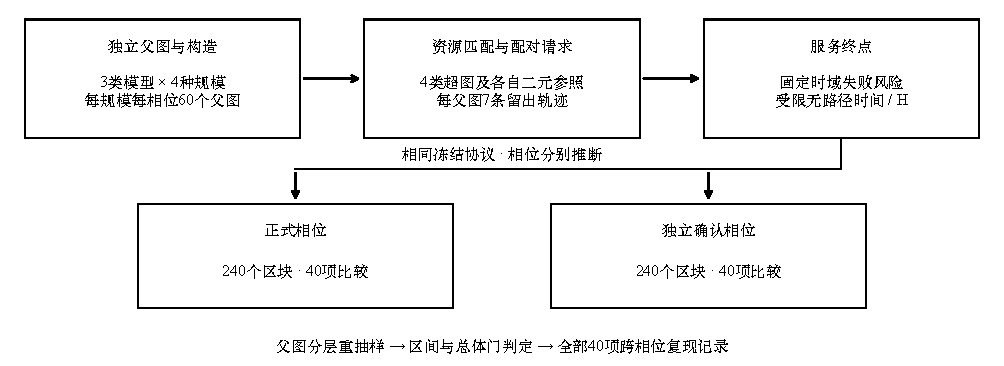
\includegraphics[width=170mm]{figures/figure-1-design.pdf}

\caption{资源匹配评估与独立确认流程。每规模每相位含60个独立父图；同一父图内7条留出轨迹为嵌套测量，两相位分别推断。}\label{fig:1}

\end{figure*}

\subsection{主要终点及配对效应}

主要终点为归一化受限无路径时间Y和固定时域失败指示F。令$T=\min(\tau_{\mathrm{np}},H)$，$\delta$表示截至H是否观察到无路径事件，则$Y=T/H$、$F=\delta$。删失观测保存$T=H$及$\delta=0$；恰在H发生事件时T同为H，但$\delta=1$。因此，两个终点分别反映首次服务中断的相对时间与观测期内是否发生中断。


对于构造族f及其$K_f$个二元参照，任一终点$Z\in\{Y,F\}$的配对差定义为



\begin{equation}
\begin{aligned}d_f^{(Z)}&=Z_f-\frac{1}{K_f}\sum_{k=1}^{K_f}Z_{f,k}^{(B)},\\d_{\mathrm{global}}^{(Z)}&=\frac{1}{4}\sum_f d_f^{(Z)}.\end{aligned}
\label{eq:13}\end{equation}


Y的差值为正、F的差值为负时表示有利方向。F是“截至H至少出现一次全局不可行请求”的指示，不是全部请求的失败比例；两组F均值之差为绝对概率差，不解释为相对下降百分比。总体对比对4类构造等权，奇数预算所增加的二元参照不提高该构造的权重。


\noindent\textbf{命题2} 对于从1开始的离散请求时钟，归一化受限无路径时间的期望等于时域内离散生存概率的平均值，即\par


\begin{equation}
\begin{aligned}\mathbb E[Y]&=\frac{1}{H}\sum_{t=0}^{H-1}\Pr(\tau_{\mathrm{np}}>t),\\\mathbb E[F]&=\Pr(\tau_{\mathrm{np}}\leq H).\end{aligned}
\label{eq:14}\end{equation}


\noindent\textbf{证明} 对任一正整数首次事件时间，或观测域内未发生事件的情形，受限时间都等于从0至H$-$1各时点“事件尚未发生”指示量之和。有限求和后取期望即得第一式；第二式由F的定义直接得到。该恒等式不依赖扩散近似，也不需要把未观测事件补成一个假定失效时刻。\par

两个终点由此具有互补性。风险只反映H之前是否发生首次事件，不区分事件发生较早还是较晚；受限时间利用时域内发生位置，但对恰在H发生与截至H未发生均取1。若只报告其中一项，可能丢失另一项所含信息。本文分别推断这两个事先确定的终点，不在看到数据后选取更有利的一项，也不据二者均有利进一步断言整个生存曲线处处占优。


\subsection{分层推断与复现准则}

先在每个父图区块内分别求4条同分布轨迹和3条偏移轨迹的平均差，再按4$:$3合并，得到1个父图观测。每个规模先求3个模型层内的均值，再对层均值等权平均。由此，每相位、每规模的独立重复数为60，轨迹数、构造数及二元参照数均不计作额外独立父图。


为明确重复单位，令 $d_{m,i,r,f}^{(Z)}$ 为模型层m内第i个父图、第r条轨迹、构造族f的配对差，令同分布和偏移轨迹集合分别为 $\mathcal R_0$ 与 $\mathcal R_1$。一个父图观测为



\begin{equation}
\begin{aligned}D_{m,i,f}^{(Z)}={}&\frac{4}{7}\frac{1}{4}\sum_{r\in\mathcal R_0}d_{m,i,r,f}^{(Z)}\\&+\frac{3}{7}\frac{1}{3}\sum_{r\in\mathcal R_1}d_{m,i,r,f}^{(Z)}.\end{aligned}
\label{eq:15}\end{equation}


因此，在当前4条与3条的固定设计中，两步汇总等于7条轨迹配对差的平均，但保留了两个负载范围的清晰定义。对于任一规模，构造族的目标均值估计为



\begin{equation}
\widehat\Delta_f^{(Z)}=\frac{1}{3}\sum_{m=1}^{3}\frac{1}{20}\sum_{i=1}^{20}D_{m,i,f}^{(Z)}.
\label{eq:16}\end{equation}


采用父图分层聚类bootstrap，各层每次有放回抽取20个父图，进行20000次重抽样，根种子为2026081003。同一局部层级中的5项对比共享重抽样索引。2个终点与4种规模组成8个局部层级，每层级包含1项总体对比和4项构造族对比，共40项预定比较。只有对应总体区间完全位于有利方向，构造族比较才具有确认性解释。


冻结的Bonferroni分配在每相位40项比较上采用95\%名义家族置信水平。8个局部层级各含5项比较，每个局部家族的名义水平为159/160；单个校正区间的名义水平为799/800，每侧经验尾概率为1/1600。区间取20000个重抽样值排序后的第13和第19988个值。该percentile bootstrap程序未证明有限样本精确覆盖率；区间及门控均按未舍入的精确分数判断。


总体比较须在两相位中均得到有利区间才满足独立确认；构造族比较还要求两相位对应总体门均开启。两相位分别推断、不合并样本，95\%的家族水平分别适用于每相位40项区间，不作为跨相位80项区间的联合保证。


\subsection{删失、成本与计算复现}

下分位水平$q=0.10$仅用于事件覆盖诊断。一个父图只有在源超图及其全部二元参照的事件观测比例均不低于0.10时才通过；某个相位、规模、模型、构造族和负载范围组成的单元，须全部父图通过才标记为完全覆盖。本研究不据此估计数值化的0.10停止时间分位数。


13项描述指标的完整定义见随稿补充说明。关键指标为关联坐标平均余额份额偏差$B(x)$及每次尝试的二次协调暴露量$Q$：
\[
\begin{aligned}
B(x)&=\frac1L\sum_{e\in\mathcal E}\sum_{v\in e}\left|\frac{x_{e,v}}{C_e}-\frac1{|e|}\right|,\\
Q&=\frac1H\sum_{t:A_t=1}\sum_{e\in P_t}|e|^2.
\end{aligned}
\]
其中$e\in P_t$指路径经过的超边。初末失衡分别为$B(x(0))$和$B(x(H))$；$B$依赖超边规模，不能作规模无关的均衡性排序。$Q$不同于训练项$O$中的成员对计数。瓶颈余额量为$H^{-1}\sum_{t:A_t=1}b(P_t,q_t)$，拒绝贡献0，值低不必然有利。简单路径下跳数与经过超边数相等。信令槽位和独立参与人数分别累计路径超边的成员数之和与成员并集大小，再除以$H$；它们不是实测时延或费用。


成本归一化使用尝试次数，而非仅成功请求次数。这一口径保持各配对变体面对相同业务时域，但也意味着成本差可能同时受路径结构和接受模式影响。例如，更多请求成功的变体可能产生更多执行协调活动；某个变体较早失败也不代表它在提供同等服务时成本更低。故成本分量与可靠性必须联合阅读，不能把单位尝试计数直接转化为单位成功支付费用。


每个区块绑定拓扑、初态、请求轨迹及路由选择的SHA-256指纹，并经冻结输入精确再生核对。正式相位完成后先生成其统计证据；2026年8月30日的就绪记录已绑定该证据，随后以不含科学终点的就绪凭证进入确认相位。确认相位完成后生成确认及跨相位证据，再按归档流程独立重放核验。分析使用可恢复检查点；原始区块、运行记录、全部比较、描述性投影及图表源数据均保留。


分析模式及复现状态机在正式相位已完成15个区块后、正式推断前补充，当时仅查看一条留出记录以识别字段结构，未计算汇总效应或区间。后续内存与并行执行修订改变进程划分及读取方式，保持冻结输入、模拟代码、终点和推断规则。该时间顺序作为方法修订披露，而不追溯表述为全部在最初运行前完成。


\section{结果与分析}

\subsection{资源匹配下的总体服务差异}

两相位均完成全部240个父图区块，形成完整的合成网络证据。8项总体比较均满足独立确认准则，具体效应和校正区间见表1，图2展示两相位估计及区间的位置。正式相位在30、60、120和240节点下的失败风险差依次为$-$0.425、$-$0.559、$-$0.701和$-$0.805；确认相位对应为$-$0.449、$-$0.575、$-$0.693和$-$0.787。确认相位240节点的估计表示固定时域内首次无路径事件的发生概率平均相差$-$0.787，即$-$78.7个百分点，不表示失败风险相对下降78.7\%。


\begin{table*}[t]\centering
\caption{总体配对效应及多重比较校正区间}\label{tab:1}
\small\begin{tabular*}{\textwidth}{@{\extracolsep{\fill}}lccc}\toprule
终点 & 节点数 & 正式相位估计［区间］ & 确认相位估计［区间］\\\midrule
失败风险 & 30 & $-0.425\;[-0.478, -0.371]$ & $-0.449\;[-0.506, -0.393]$\\
失败风险 & 60 & $-0.559\;[-0.612, -0.507]$ & $-0.575\;[-0.628, -0.519]$\\
失败风险 & 120 & $-0.701\;[-0.754, -0.645]$ & $-0.693\;[-0.745, -0.646]$\\
失败风险 & 240 & $-0.805\;[-0.842, -0.765]$ & $-0.787\;[-0.829, -0.742]$\\
受限时间$/H$ & 30 & $0.192\;[0.158, 0.230]$ & $0.216\;[0.183, 0.249]$\\
受限时间$/H$ & 60 & $0.307\;[0.266, 0.346]$ & $0.305\;[0.266, 0.344]$\\
受限时间$/H$ & 120 & $0.437\;[0.401, 0.474]$ & $0.441\;[0.398, 0.485]$\\
受限时间$/H$ & 240 & $0.566\;[0.531, 0.600]$ & $0.562\;[0.530, 0.594]$\\
\bottomrule\end{tabular*}
\par\smallskip\footnotesize 每相位每行含60个独立父图；区间为父图分层percentile bootstrap经Bonferroni校正的区间，每相位40项比较的名义家族水平为95\%。风险差为负、受限时间差为正表示有利方向。
\end{table*}

归一化受限无路径时间的正式相位差值为0.192、0.307、0.437和0.566，确认相位为0.216、0.305、0.441和0.562。两相位各规模区间均位于正侧，表明在共同请求时域内，超图构造相对于其匹配二元参照较晚出现首次服务中断，或更常保持至观测终点。这里的时间以请求序号计量，不能直接换算为秒，也不代表无限时间的网络寿命。


\begin{figure*}[t]\centering

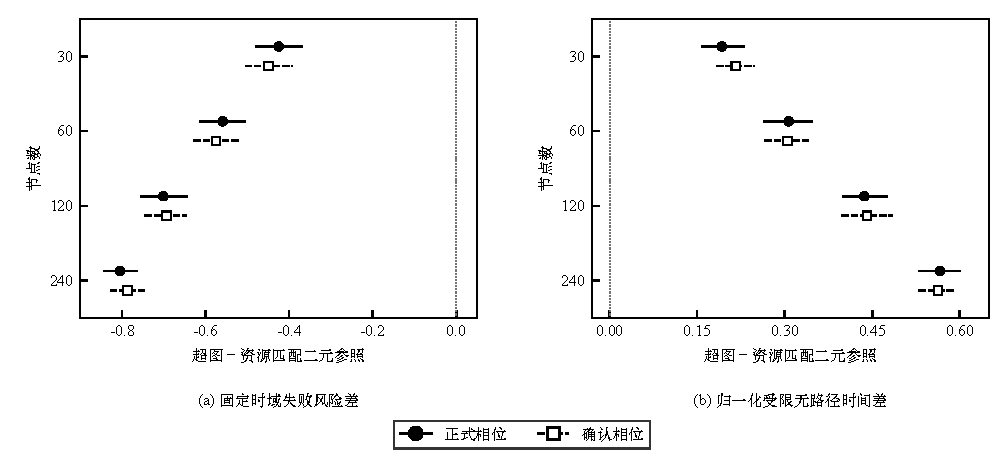
\includegraphics[width=170mm]{figures/figure-2-global-contrasts.pdf}

\caption{两相位总体服务效应。(a)固定时域失败风险差；(b)归一化受限无路径时间差。圆点为正式相位，方点为确认相位；水平线为父图分层percentile bootstrap经Bonferroni校正的区间，每相位40项比较的名义家族水平为95\%；虚线为零差。每个估计含60个父图，重抽样20000次。}\label{fig:2}

\end{figure*}

随规模增大，总体失败风险差的绝对值与归一化受限时间差均呈增大的描述性趋势。不过，规模变化同时改变边数与请求时域，且没有为规模间差异另设确认性检验。因此，该趋势只描述4个预定规模下的结果，不构成关于任意规模单调改善的定理。


\subsection{构造族与父图结构的复现}

两相位全部总体门均开启。需求感知超图、FHS3、FHS5和NCH在2个终点、4种规模上的32项构造族比较，校正区间均在两相位中位于有利方向；加上8项总体比较，40项记录均满足独立确认准则。完整状态矩阵见图3，未出现仅正式相位、仅确认相位或两相位均未通过的记录。


\begin{figure*}[t]\centering

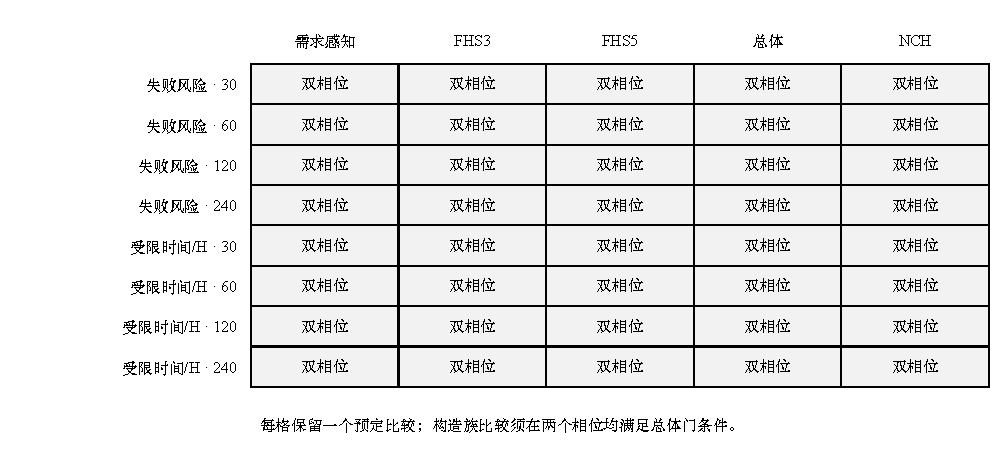
\includegraphics[width=170mm]{figures/figure-3-replication-matrix.pdf}

\caption{全部40项比较的跨相位复现。每格对应一项预定比较。“双相位”表示校正区间均有利且适用的总体门均开启；不表示超图构造之间的两两排序。}\label{fig:3}

\end{figure*}

按父图模型进一步展开，每相位5类对比（含总体）、4种规模和3个模型组成60个描述性单元；失败风险均值全部为负，归一化受限时间均值全部为正。方向一致性覆盖BA、ER-GNM和固定边数SBM，但这些分层均值不构成新增的独立检验，也未验证3类模型的效应相等。各单元20个父图的原值、均值及范围保存在源数据中。


表2列出总体失败风险的全部规模—模型层均值。30节点时，正式相位BA、ER-GNM和固定边数SBM层分别为$-$0.606、$-$0.319和$-$0.350，确认相位分别为$-$0.596、$-$0.342和$-$0.410；240节点时，正式相位分别为$-$0.946、$-$0.772和$-$0.696，确认相位分别为$-$0.943、$-$0.709和$-$0.709。层均值在方向上保持一致，但量级有差异，说明总体均值不应被理解为每种父图结构具有相同改善程度。


\begin{table}[t]\centering
\caption{总体失败风险差的父图模型分层均值}\label{tab:2}
\small\begin{tabular*}{\columnwidth}{@{\extracolsep{\fill}}clrr}\toprule
节点数 & 父图模型 & 正式 & 确认\\\midrule
30 & BA & $-0.606$ & $-0.596$\\
30 & ER-GNM & $-0.319$ & $-0.342$\\
30 & SBM & $-0.350$ & $-0.410$\\
60 & BA & $-0.788$ & $-0.815$\\
60 & ER-GNM & $-0.477$ & $-0.482$\\
60 & SBM & $-0.412$ & $-0.427$\\
120 & BA & $-0.959$ & $-0.939$\\
120 & ER-GNM & $-0.627$ & $-0.595$\\
120 & SBM & $-0.518$ & $-0.546$\\
240 & BA & $-0.946$ & $-0.943$\\
240 & ER-GNM & $-0.772$ & $-0.709$\\
240 & SBM & $-0.696$ & $-0.709$\\
\bottomrule\end{tabular*}
\par\smallskip\footnotesize 每格含20个父图；SBM为固定边数SBM。仅为描述性均值，不是新增显著性检验。
\end{table}

模型内还存在个体差异。例如，正式相位120节点的FHS3在ER-GNM层中，父图风险差最大值为0.071，受限时间差最小值为$-$0.132，均提示至少存在方向不利的父图记录；这两项极值不必来自同一个父图。层平均有利、校正区间有利与每个父图均有利是不同命题。报告这种异质性有助于避免将群体比较误读为任意给定拓扑上的服务保证。


上述结构分层没有单独建立模型之间效应差的确认性区间，也没有在控制其他结构特征后识别某个图统计量的因果作用。因此，不能由BA层的描述性差值较大，就推断偏好连接是唯一机制；同样不能由各模型方向一致，声称社区瓶颈或高度节点对性能没有影响。当前分层结果提供了后续机制检验应关注的差异，而非替代机制检验。


\subsection{删失覆盖与需求感知构造的活动范围}

服务效应的跨相位复现并不意味着所有停止时间特征都已可识别。每相位96个覆盖诊断单元中，仅2个满足所有父图及其全部参照的$q=0.10$事件覆盖规则，均为FHS3在固定边数SBM、同分布范围、120和240节点下的单元。正式相位有34个单元、确认相位有24个单元没有任何父图通过联合覆盖规则，其余为部分覆盖。这些数目统计的是单元，同一父图会在不同构造和负载范围内重复出现。本研究未报告0.10分位数的数值估计。


需求感知训练在4种递增规模下，分别改变正式相位60个父图中的33、21、5、1个种子拓扑，确认相位对应为34、16、13、1个。到240节点时，两相位的改变组均仅有1个父图，分别来自BA和ER-GNM，其余两个模型层为空，因而无法形成等模型权重的改变组均值。未改变组在两相位的失败风险均值差分别为$-$0.922和$-$0.898，归一化受限时间均值差为0.638和0.647。


上述分组仍然是最终超图相对于二元参照的描述性比较，不是改变前后拓扑的配对因果效应。尤其在大规模下，改变组过小，当前数据不能支持“训练带来额外服务收益”的结论。结果反而提示，需要将种子本身的多方结构效应与局部搜索的增量作用分开检验。


\begin{table}[t]\centering
\caption{需求感知搜索的改变与未改变父图数}\label{tab:3}
\small\begin{tabular*}{\columnwidth}{@{\extracolsep{\fill}}crrrr}\toprule
&\multicolumn{2}{c}{正式相位}&\multicolumn{2}{c}{确认相位}\\
节点数&改变&未改变&改变&未改变\\\midrule
30 & 33 & 27 & 34 & 26\\
60 & 21 & 39 & 16 & 44\\
120 & 5 & 55 & 13 & 47\\
240 & 1 & 59 & 1 & 59\\
\bottomrule\end{tabular*}
\par\smallskip\footnotesize 每规模每相位共60个父图；改变相对于FHS5种子定义，不表示服务改善。
\end{table}

表3同时报告改变数和母体数。未改变不等于未训练：搜索可在检查提案后保留种子；改变也不证明留出服务提高。120节点两相位分别改变5和13个拓扑，该差异不能直接解释为算法稳定性指标。


事件较少可能增大受限时间，却同时削弱低分位停止时间的识别。覆盖不足既不等于实验失败，也不能被有利服务效应抵消。本文保留风险和受限时间终点，将$q=0.10$限于诊断，不延长或筛选部分轨迹补救覆盖。


\subsection{服务收益与协调开销}

每相位保留4种规模与4类源构造组成的16个等模型均值单元及全部13项描述指标。全部16个单元的节点对覆盖与覆盖重数差均为正，初末$B$值及终态零坐标比例差均为负；$B$值较低不等价于规模无关的余额更均衡。按尝试归一的跳数（与经过超边数相同）及瓶颈余额量差均为负；信令槽位、独立参与人数及$Q$差均为正。两项最优路径重数指标的差值符号随单元变化。这些方向是描述性结果，不构成13项独立的改善证据。


二次协调暴露量差的正式相位范围为6.857～316.591，确认相位为6.886～306.536。该结果说明，按尝试计的路径长度较低并不保证协调暴露量较低。现有联合比较未隔离节点对覆盖、超边规模与接受模式，余额偏差指标又受规模影响，因此不能据此识别服务差异的机制。工程设计需同时评估服务事件和多方协调分量。


正式与确认相位记录的区块生成耗时之和分别为294.922和264.831区块小时，精确验证耗时之和为340.418和299.433区块小时。这里累加的是各区块实际经历的时长，既非端到端墙钟时间，也非CPU小时；后续相位推断和描述性投影耗时不在其中，因此不能用作并行加速比。两相位运行记录均为Windows AMD64上的CPython 3.12.13，现有摘要未提供全程峰值内存。


\subsection{结果之间的一致性与解释边界}

总体差异随规模增大的趋势还与观测时域$H=12n$共同变化。不同规模比较的既是不同节点数量，也是不同时域下的归一化事件过程；除以H统一了无量纲表达，并不把各规模变成相同的业务实验。要判断纯粹的规模效应，需要另行固定时域或设计规模与时域的交叉实验，当前确认结论仅针对各个已声明规模分别成立。


\section{讨论}

\subsection{从局部余额事件到网络服务评价}

结果表明，在所设资金、参与关系、负载和路由约束下，超图构造相对于二元参照的服务效应具有跨相位一致性。该证据将多超边状态更新、全局可行路径与独立父图重复结合起来，适用于当前受控比较，尚不足以推广至所有业务和协议。


多超边扩展的关键不只是增加状态维数，还包括改变停止集合的含义。余额触零由一个关联坐标决定，无路径则由当前请求与全部可行路径共同决定；后者可能在所有坐标仍为正时发生。将两层分开，使理论分析能够明确处理状态可行域与守恒性质，使实验能够在指定协议下检验服务事件，避免通过更换事件名称制造形式上的理论推广。


\subsection{资源公平性与服务成本取舍}

资源匹配未固定节点参与度序列和节点对覆盖，这些差异属于被比较的结构组成。奇数预算的上下参照均值则具有预算邻域含义，不对应实际运行的“平均网络”。因此，匹配不意味着全部成本分量相同。


较少的经过超边数与较高的协调暴露量并不矛盾。一次经过较大超边的局部转移，可以在较少网络跳数内连接更多候选成员，同时涉及更多潜在协调关系。若部署环境主要受通信往返次数限制，路径长度可能更重要；若受参与方签名、故障协调或隐私要求限制，参与规模可能更重要。当前实验未测量这些实现级代价，因此只能指出取舍方向，不能给出统一最优超边规模。


\subsection{统计范围与外部有效性}

余额隐私、探测、手续费、重试及并发占用会改变实际可行集合与拒绝原因；协调计数也不能代替实现级时延或费用。向真实部署推广需要补充信息不完备与并发协议验证。


每个模型层仅含20个父图，percentile bootstrap的尾部近似可能影响区间稳定性，多重比较分配不消除该误差。$q=0.10$覆盖不足限制了低分位分析。确认相位仍采用相同合成机制，无法据此估计真实闪电网络的失败率。


\subsection{可验证的后续研究方向}

后续可增加需求感知构造相对于FHS5种子的直接配对消融，检验搜索增量；在不同请求时域与资金预算下验证趋势；测量多方协调对应的通信和锁定时延。


\section{结束语}

围绕多超边支付网络的持续服务问题，建立了资源匹配、状态化配对执行和父图分层独立确认相结合的评估方法。该方法将首次无可用路径与首次余额耗尽分开记录，以固定时域失败风险和归一化受限无路径时间评价服务，在共同资金与参与关系约束下比较4类超图构造及其二元参照。两独立相位各240个父图区块的结果表明，全部40项预定比较满足复现准则，观察到的服务收益同时伴随更高的多方协调暴露量。结论适用于当前合成父图、负载、资金和余额感知路由设置，为进一步研究信息约束及实现成本提供了可复用的比较基础。


\section*{数据与代码}

实验代码、配置、运行与验证记录、相位分析证据和图表源数据保存在项目仓库中（\url{https://github.com/megumidaisuki-jth/secondaryexploration}）。正文数字可追溯至完整比较登记表和描述性汇总。本稿只使用已完成的合成网络数据，公开拓扑截面不参与当前结果。持久化归档标识及最终代码、数据许可证将在投稿材料中补充。


\begin{thebibliography}{99}\small\raggedright\setlength{\itemsep}{2pt}

\bibitem{r1} PAPADIS N, TASSIULAS L. Blockchain-based payment channel networks: challenges and recent advances[J]. IEEE Access, 2020, 8: 227596-227609. DOI: 10.1109/ACCESS.2020.3046020.

\bibitem{r2} 徐秀, 田安琪, 何瑞雯. 基于区块链的支付信道网络：挑战与发展[J]. 通信学报, 2024, 45(Z1): 97-104. DOI: 10.11959/j.issn.1000-436x.2024217.

\bibitem{r3} SIVARAMAN V, VENKATAKRISHNAN S B, RUAN K, et al. High throughput cryptocurrency routing in payment channel networks[C]//Proceedings of the 17th USENIX Symposium on Networked Systems Design and Implementation. Santa Clara, USA: USENIX Association, 2020: 777-796.

\bibitem{r4} WANG P, XU H, JIN X, et al. Flash: efficient dynamic routing for offchain networks[C]//Proceedings of the 15th International Conference on Emerging Networking Experiments and Technologies. Orlando, USA: ACM, 2019: 370-381. DOI: 10.1145/3359989.3365411.

\bibitem{r5} KHALIL R, GERVAIS A. Revive: rebalancing off-blockchain payment networks[C]//Proceedings of the 2017 ACM SIGSAC Conference on Computer and Communications Security. Dallas, USA: ACM, 2017: 439-453. DOI: 10.1145/3133956.3134033.

\bibitem{r6} AVARIKIOTI G, WANG Y, WATTENHOFER R. Algorithmic channel design[C]//29th International Symposium on Algorithms and Computation. Dagstuhl: Schloss Dagstuhl–Leibniz-Zentrum für Informatik, 2018, 123: 16:1-16:12. DOI: 10.4230/LIPIcs.ISAAC.2018.16.

\bibitem{r7} KHAMIS J, ROTTENSTREICH O. Demand-aware channel topologies for off-chain payments[C]//2021 International Conference on COMmunication Systems \& NETworkS. Piscataway: IEEE, 2021: 272-280. DOI: 10.1109/COMSNETS51098.2021.9352899.

\bibitem{r8} KHAMIS J, KOTZER A, ROTTENSTREICH O. Topologies for blockchain payment channel networks: models and constructions[J]. IEEE/ACM Transactions on Networking, 2024, 32(6): 4781-4797. DOI: 10.1109/TNET.2024.3445274.

\bibitem{r9} PODIATCHEV Y, ORDA A, ROTTENSTREICH O. Survivable payment channel networks[J]. IEEE Transactions on Network and Service Management, 2024, 21(6): 6218-6232. DOI: 10.1109/TNSM.2024.3456229.

\bibitem{r10} KOTZER A, LADÓCZKI B, TAPOLCAI J, et al. Addressing scalability issues of blockchains with hypergraph payment networks[J]. IEEE Transactions on Network and Service Management, 2025, 22(3): 2427-2440. DOI: 10.1109/TNSM.2025.3542960.

\bibitem{r11} CORCORAN P, LEWIS R. Path planning in payment channel networks with multi-party channels[J]. Distributed Ledger Technologies: Research and Practice, 2025, 4(4): 1-14. DOI: 10.1145/3702248.

\bibitem{r12} HUANG L, HUO C, GE C, et al. AERO: an adaptive and efficient routing for off-chain payment channel networks[J]. Computer Networks, 2025, 257: 111009. DOI: 10.1016/j.comnet.2024.111009.

\bibitem{r13} CHATTERJEE K, KŘIŠŤAN J M, SCHMID S, et al. Boosting payment channel network liquidity with topology optimization and transaction selection[C]//39th International Symposium on Distributed Computing. Dagstuhl: Schloss Dagstuhl–Leibniz-Zentrum für Informatik, 2025, 356: 23:1-23:22. DOI: 10.4230/LIPIcs.DISC.2025.23.

\bibitem{r14} PICKHARDT R. A mathematical theory of payment channel networks[EB/OL]. (2026-01-08)[2026-09-29]. \url{https://arxiv.org/abs/2601.04835}. 预印本.

\bibitem{r15} YU W, XU M, ZHANG Y, et al. Starfish: rebalancing multi-party off-chain payment channels[EB/OL]. (2026-09-21)[2026-09-29]. \url{https://arxiv.org/abs/2504.20536v2}. 修订预印本.

\end{thebibliography}\section*{作者简介}

【作者姓名、出生年、学位、单位、职称及主要研究方向待填；照片由作者提供】


\end{document}
